%%%%%%%%%%%%%%%%%%%%%%%%%%%%%%%%%%%%%%%%%%%%%%%%%%%%%%%%%%%%%%%%%%%%%%%%%%
 %																		%
 %	Plantilla Latex para presentación del proyecto de curso				%
 %	Programación de Aplicaciones para Internet y la Nube					%
 %																		%
 %	Creada por: Duván Pardo, Wilson López								%
 %																		%
 %	Versión: 0.2															%
 %	Dapardoc@gmail.com ; Wilrilo@gmail.com								%
 %																		% 
 %	Se requieren los archivos  presentación.bbl							% 
 %	El directorio Imagenes que contiene: escudoud.pdf,ECHO_OFF	 		%  
 %																		%
%%%%%%%%%%%%%%%%%%%%%%%%%%%%%%%%%%%%%%%%%%%%%%%%%%%%%%%%%%%%%%%%%%%%%%%%%%

\documentclass[11pt]{beamer}					% Describe el tipo de documento, y el tamaño de la letra del texto
\usepackage[utf8]{inputenc}					% Define codificación para que permita caracteres latinos (acentos)
\usepackage[spanish,activeacute]{babel} 		% Paquete para poder escribir con tildes y otros caracteres especiales

\usepackage{amsmath}							% paquete para expresiones matemáticas
\usepackage{amsfonts}						% paquete para escritura de ecuaciones 
\usepackage{amssymb}							% paquete para caracteres especiales para ecuaciones 

\usepackage{svg}								% Se utiliza para incluir imágenes vectorizadas en el documento (.pdf)
\usepackage{hyperref}						% Para hipervinculos

\usepackage{lmodern}							% http://ctan.org/pkg/lm
\usepackage{listings}						% Para el código fuente
\usepackage{xcolor}							% Para el color en código fuente
\usepackage{graphicx}						% Para incluir imágenes
\graphicspath{{Imagenes/}}					% Directorio de imágenes

\bibliographystyle{apalike} 					% Bibliografia tipo APA

\definecolor{limegreen}{RGB}{50,100,50}		% Definición de color
\lstdefinestyle{base}{						% Para el color en código fuente
	language=C,
	emptylines=1,
	breaklines=true,
	showspaces=fasle,
	showstringspaces=false,
	extendedchars=true,
	basicstyle=\ttfamily\color{black},
	moredelim=**[is][\color{limegreen}]{'}{'},
	moredelim=**[is][\color{blue}]{&}{&},
}				
\lstset{numbers=left, numberstyle=\tiny, stepnumber=1, numbersep=5pt}	% Muestra numeración al lado del código

\mode<presentation>{	
	\usetheme{Frankfurt}		
% Temas: AnnArbor,Antibes, Bergen, Berkeley, Berlin, Boadilla, boxes, CambridgeUS, Copenhagen, Darmstadr, default, Dresden, Frankfurt*, Goettingen, Hannover, LLmenau, JuanLesPins, Luebeck, Madrid, Malmoe, Marburg, Montpellier, PaloAlto, Pittsburgh, Rochester, Singapore, Szeged, Warsaw.	
	\usecolortheme{orchid}	
% Colores:albatross, beaver, beetle, crane, default, dolphin, dove, fly, lily, orchid*, rose, seagull, seahorse, sidebartab, structure, whale, wolverine.	 
}

\logo{
\includegraphics[scale=0.04]{escudoud}}
\title{Plantilla para presentación \\ --- \\ Título y Subtitulo}
\author{Estudiante(s): Duván Pardo, Wilson López}
\institute[UD]{Universidad Distrital Francisco José de Caldas}
\date{\today}

\begin{document}	
	
\begin{frame}[fragile]							% Diapositiva Presentación
		\titlepage 
		\begin{small}
			''Nota de la presentación''
		\end{small}
\end{frame}	

	\begin{frame}[fragile]							% Diapositiva Tabla de Contenido
		\frametitle{Índice}	
		\tableofcontents
\end{frame}	

\section{Primera Sección}
\begin{frame}[fragile]						% Primera Diapositiva
			\frametitle{Título}
			\begin{huge}
			\begin{center}
				\emph{\textit{Primera Sección}}
			\end{center}
			\end{huge}
\end{frame}	
	\subsection{Primera Sub-Sección}	
\begin{frame}[fragile]						% Segunda Diapositiva
				\frametitle{Ejemplo de bloques y código Fuente}
				\begin{block}{Primer bloque de texto}
Texto aquí
				\end{block}
				\begin{block}{Ejemplo: Código RNW}				
				\begin{tiny}\begin{lstlisting}[frame=single,style=base]				
& \documentclass & {article}
& \usepackage[utf8] & {inputenc}
& \begin & {document}
&  \title & {Ejemplo Publicacion de Informes}
&  \author & {Duvan Pardo}
&  \maketitle &  
  A continuacion la grafica de la funcion seno (x) para -$ &\pi& < x < &\pi& $  
  '<<setup, include=FALSE>>='
		knitr::opts_chunk$set(echo = &FALSE&, message = &FALSE&, warning = &FALSE&)
  '@'
  '<<model, fig.width=4, fig.height=3, fig.align="center">>='
    plot(sin,-pi,pi,col = "green")
  '@'
\end{document}
				\end{lstlisting}	\end{tiny}	
				\end{block}			
\end{frame}	
			
\section{Segunda Sección}	
\begin{frame}[fragile]
			\frametitle{Título}
			\begin{huge}
			\begin{center}
				\emph{\textit{Segunda Sección}}
			\end{center}
			\end{huge}
\end{frame}		
		   		
    		\subsection{Segunda Sub-Sección}			
\begin{frame}[fragile]
				\frametitle{Ejemplo de imagen}							
				\begin{figure}[htb]
				\centering
					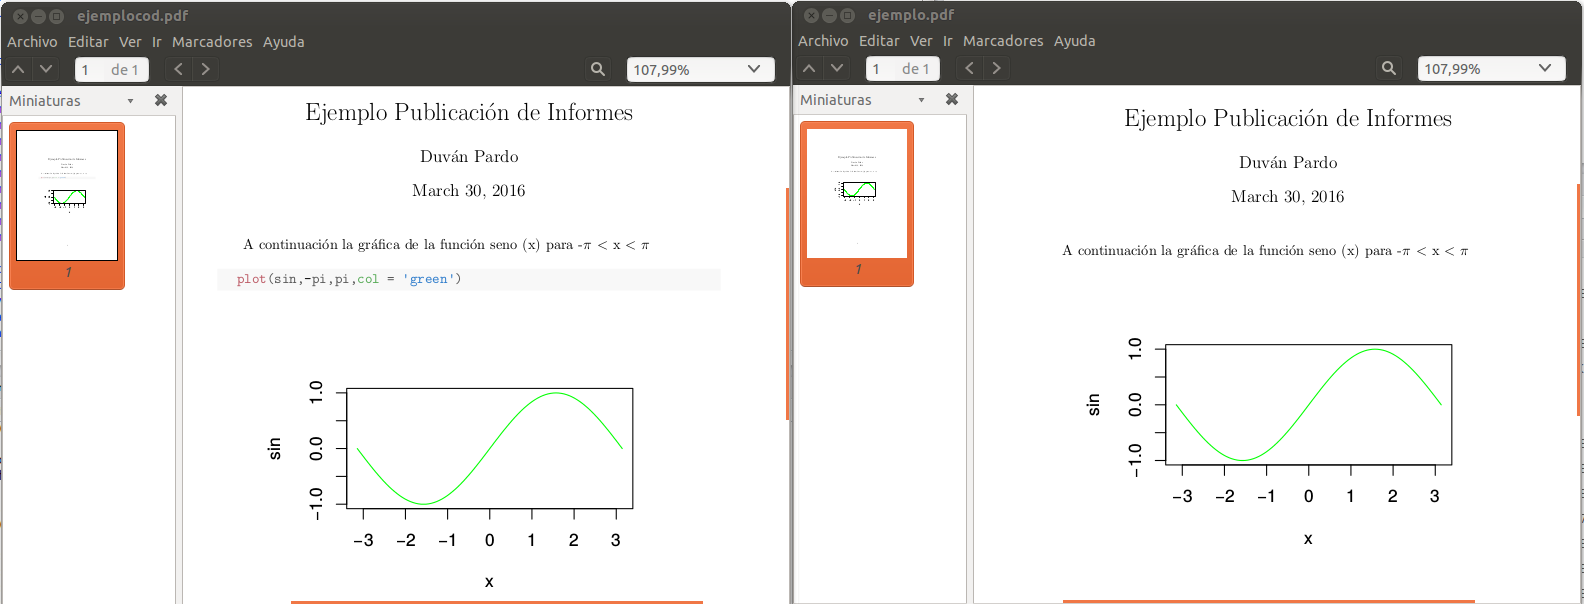
\includegraphics[scale=0.18]{ECHO_OFF}
					\caption{Comparación ocultando y sin ocultar el código.} \label{fig:ECHO_OFF}
				\end{figure}
\end{frame}
\begin{frame}[fragile]
				\frametitle{Ejemplo de imagen en un bloque}	
				\begin{block}{imágen}
					\begin{figure}[htb]
					\centering
					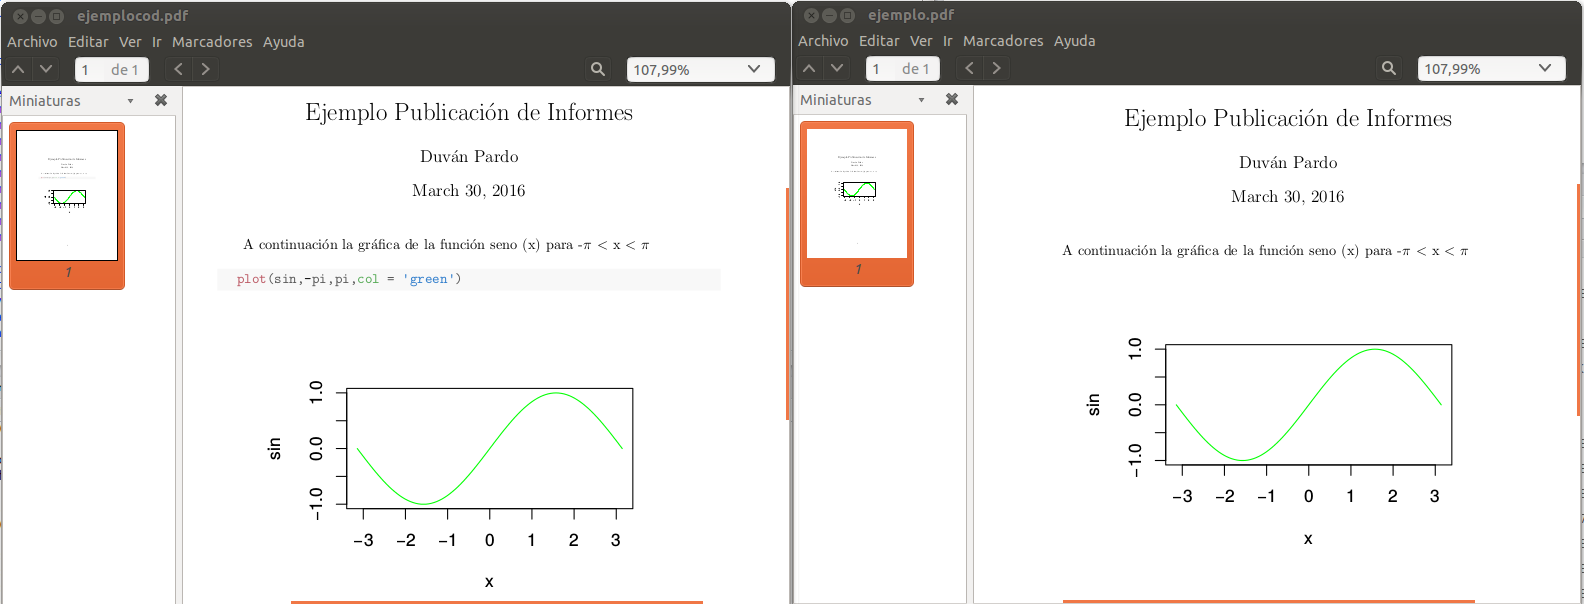
\includegraphics[scale=0.18]{ECHO_OFF}
					\caption{Comparación ocultando y sin ocultar el código.} \label{fig:ECHO_OFF1}
				\end{figure}
				\end{block}
\end{frame}
		\subsection{Tercera Sub-Sección}			
		 \begin{frame}[fragile]						% Primera Diapositiva
			\frametitle{Ejemplo con Ecuaciones y notas de pie de pagina}
\LaTeX{} es un programa para preparar documentos con el sistema de tipografías \footnote{ Según Wikipedia, la tipografía es el arte y técnica del manejo y selección de tipos, originalmente de plomo, para crear trabajos de impresión} \TeX{}.\\
\LaTeX{} fue desarrollado originalmente por Leslie Lamport en 1984 y se convirtió en el método dominante para la manipulación de \TeX. La versión utilizada para generar este documento es \LaTeXe. \newline  
  			% El siguiente código muestra la calidad de la tipografía de LaTeX
  			\begin{align}
    				E &= mc^2                              	\\
    				m &= \frac{m_0}{\sqrt{1-\frac{v^2}{c^2}}}
  			\end{align}
\end{frame}
		
\begin{frame}[fragile]						% Primera Diapositiva
			\frametitle{Título}
			\begin{block}{Ecuaciones}
				\begin{align}
					\begin{matrix}A\xrightarrow{\;\;\;f\;\;\;}B\\
					\pi\downarrow{\;\;\;\;\;}\;\;\;\uparrow{} \phi\\
					C\xrightarrow{\;\;\;g\;\;\;}D\end{matrix}
				\end{align}
				\begin{align}
					{n \choose r} = \frac{n!}{r! (n - r)!} \\
					\lim_{n \rightarrow \infty}
					\frac {n \cdot l}{2 \cdot r} = \pi
				\end{align}
			\end{block}
\end{frame}
							
\section{Bibliografía}	
%BIBLIOGRAFIA 
\begin{frame}[fragile]
		\frametitle{Bibliografía} 		
        \bibliography{Biblio} 	%Para que aparezca toda la bibliografia que citamos en el documento Biblio.bib, Informe.bbl.
       	\nocite{*}				%Para que aparezca toda la bibliografia que NO citamos en el documento, pero que utilizamos.
\end{frame}		
			
\end{document}
